\subsection{Product perspective}
Domande utili per UML:
\begin{enumerate}
    \item C'è una relazione 1:1 tra CPO e CPMS oppure un CPO è una compagnia che gestisce tante stazioni di ricarica?
    \item Mi immagino il CPMS come una periferica che ha ogni stazione a disposizione, l'UML mostra la struttura dati / funzionale del sistema eMSP, quindi non ha la facoltà di aggiornare attivamente i componenti come CPMS e socket. Vogliamo includere un'interfaccia che permetta a questi componenti di fare una richiesta al server per aggiornare i dati?\\
          Per quanto riguarda l'utilizzare un'altra interfaccia pensavo di inserire un'interfaccia che permettesse di interfacciarsi con il CPMS e con i vari sockets del modello centralizzato. In questo modo non si intaccherebbe l'interfaccia utente e ci sarebbe modo di avere un "filo" di ragionamento coerente con il modello e con la rappresentazione fisica.
    \item Il pattern più comodo per il sistema sarebbe partire sempre da una richiesta del client e poi rispondere. Mi chiedo quindi se è possibile seguire questo profilo in tutto il progetto. Per il calendario pensavo che il client (leggermente fat) potesse chiedere ogni tot al server se sarebbe un buon momento per fare rifornimento ed il server risponde.
\end{enumerate}
\begin{figure}[h!]
    \begin{center}
        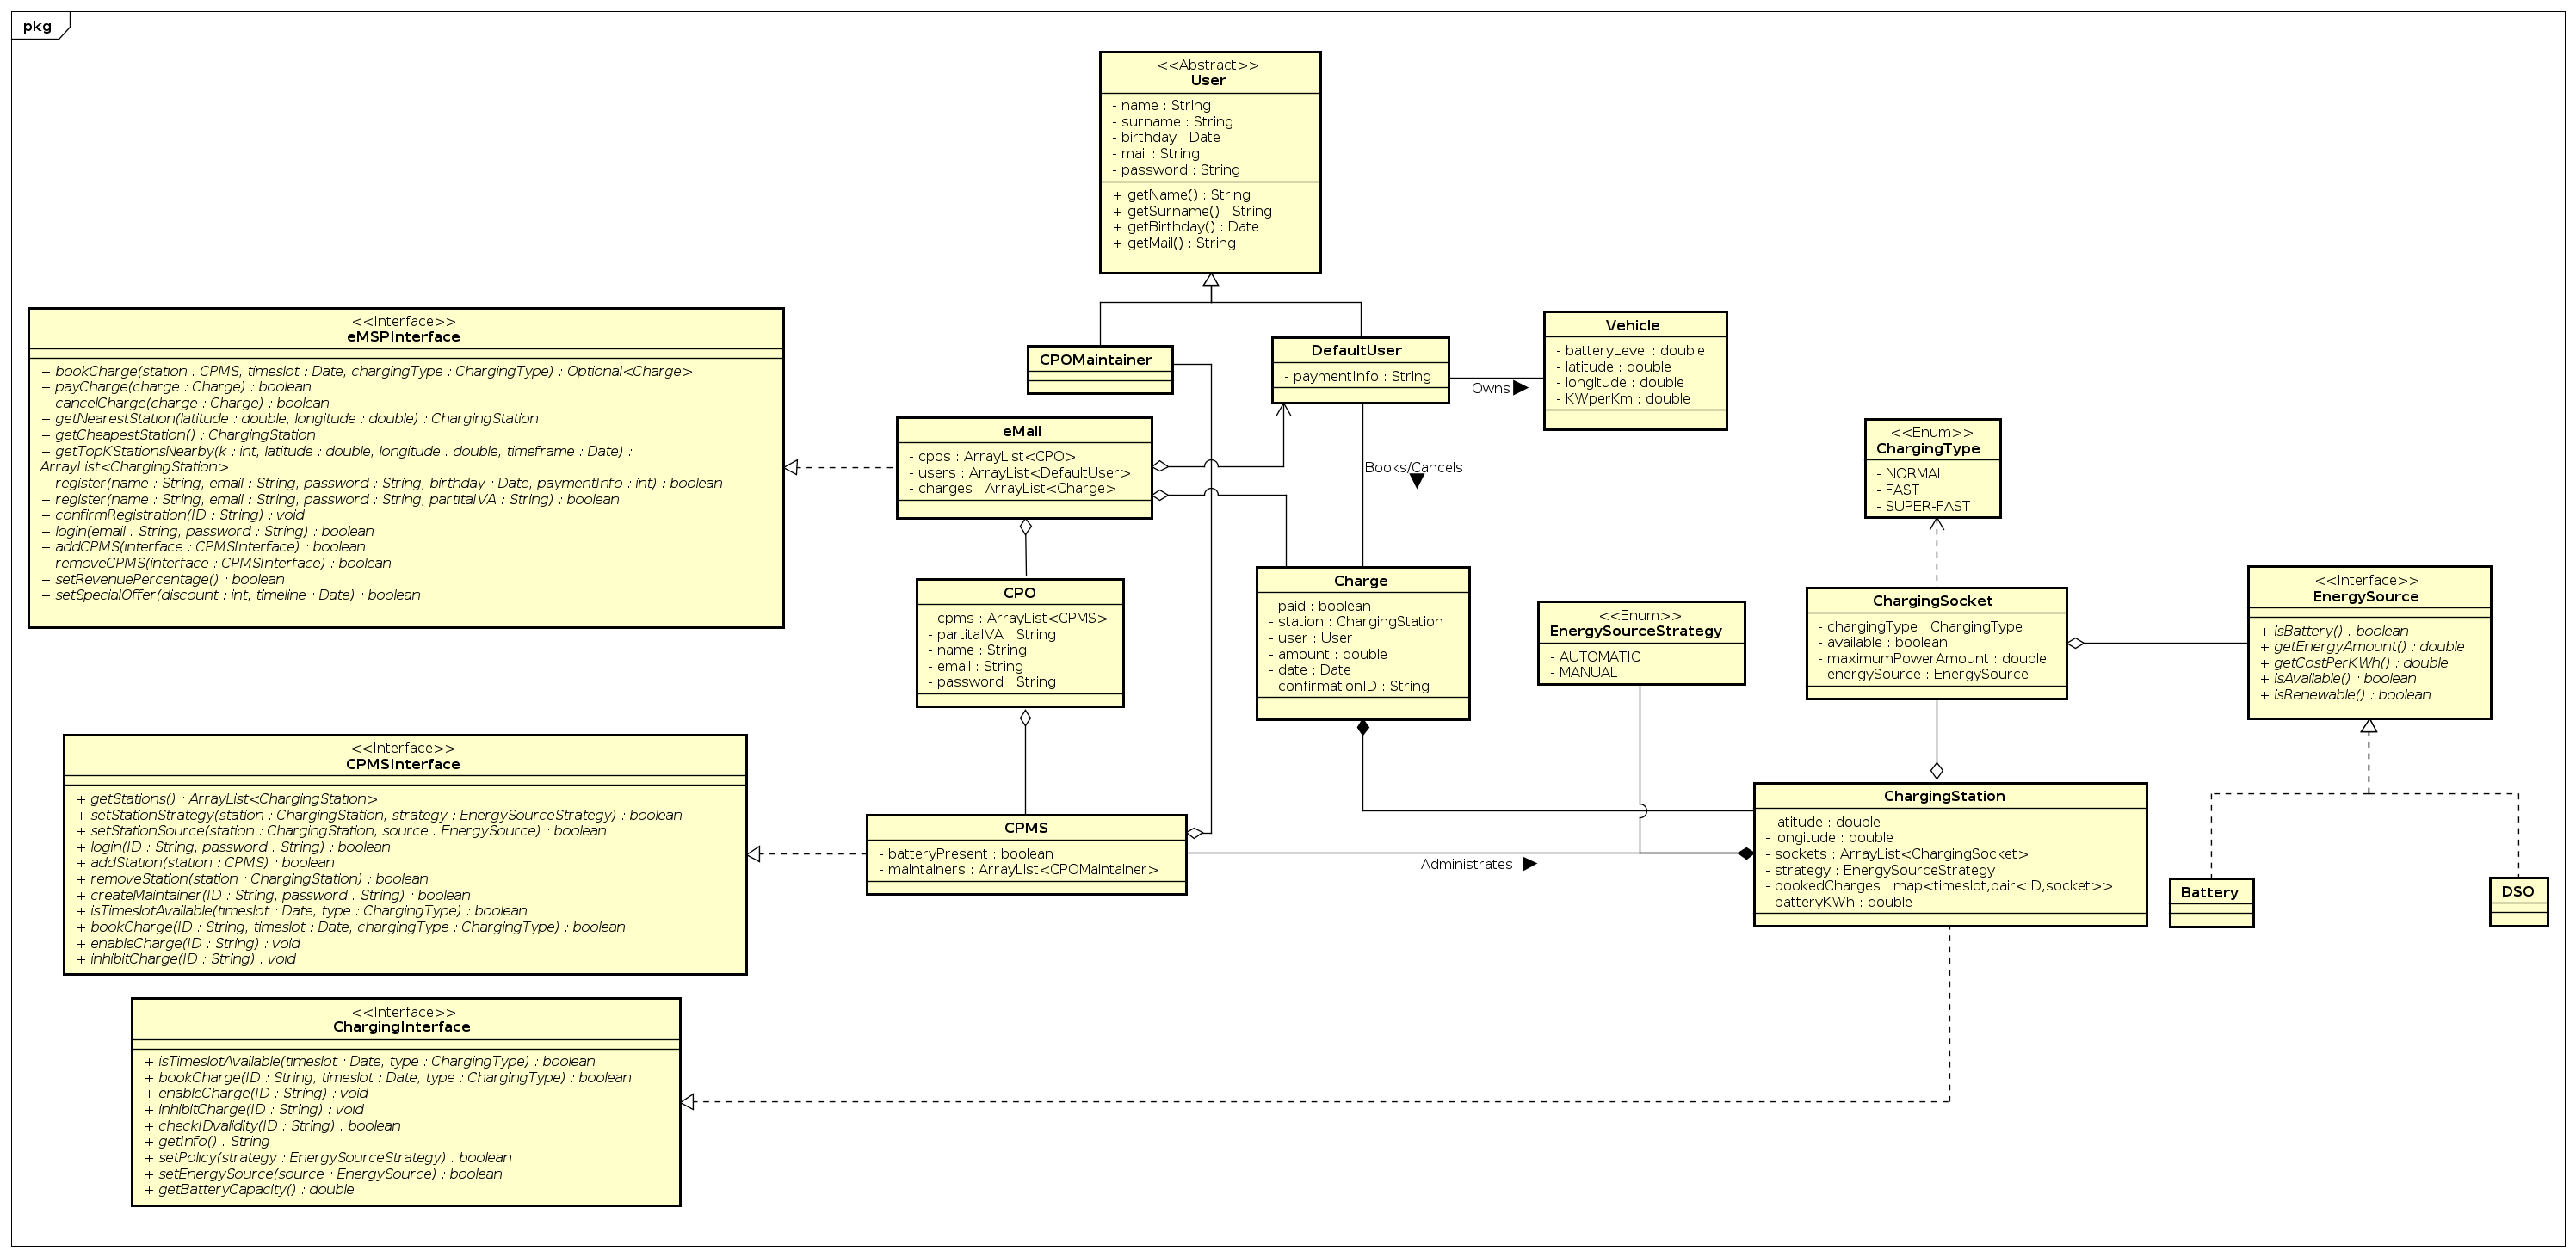
\includegraphics[keepaspectratio, width=16cm]{UML.png}
        \caption{UML}
    \end{center}
\end{figure}
\subsection{Product functions}

\subsubsection{Scenarios}
\begin{enumerate}[label=S\arabic*]
    \item User Sign up\\
          Lucy, wanting to use the system, opens the app, she is prompted to login or register, she chooses to register herself and insert her personal info (email, password, payment information), a confirmation email is sent with a link to confirm the activation of the account, if the link is clicked in the first 15 minutes the account is activated and the sign up is successful, otherwise it is considered failed and the process must be repeated.
    \item User Logs in:\\
          Lucy, after signing up, opens the up and she is prompted to insert her email, and password, if correct the login is successful and she has access to her account and the service of the apps, otherwise the login is unsuccessful and must be repeated.
    \item User search for stations
    \item User book a charge
    \item User charge the car
    \item User gets charging suggestion based on his calendar
    \item Cpo subscribe to the system
    \item Cpo updates infos about its charging stations
    \item Cpo decide the policy to be applied
    \item Cpo check internal info about the selected charging station
\end{enumerate}
\subsection{User characteristics}

\subsection{Assumptions dependencies and constraints}
\subsubsection{Assumptions}
\begin{enumerate}[label=A\arabic*]
    \item Users insert correct data in the forms
    \item Le persone non trollano
\end{enumerate}
\clearpage